% Define un comando para mostrar y copiar el texto
\newcommand{\copiabletext}[2]{%
    \href{#2}{\texttt{#1}}%
}

\begin{center}
    \centering
    \section{Introduction}
\end{center}
Welcome to the user manual of HULK, the programming language of the University of Havana. This manual is divided into 5 sections, each one dedicated to a part of the interpreter. The first section explains how to install the interpreter, the second section explains how to use the interpreter, the third section explains how to use the lexical analyzer, the fourth section explains how to use the syntax analyzer and the fifth section Explains how to use the expression evaluator.

\subsection{Start}
    \begin{itemize}
        \item To start using the interpreter, you must download the source code of the interpreter from the project's github repository. Once the source code has been downloaded, the project must be run using the `dotnet run' command from a terminal open in the project folder.
        \item Another option is to run the script which will take care of everything
        \item See previous report in \url{https://github.com/ARKye03/mini_kompiler.git}
    \end{itemize}

\begin{figure}[h]
    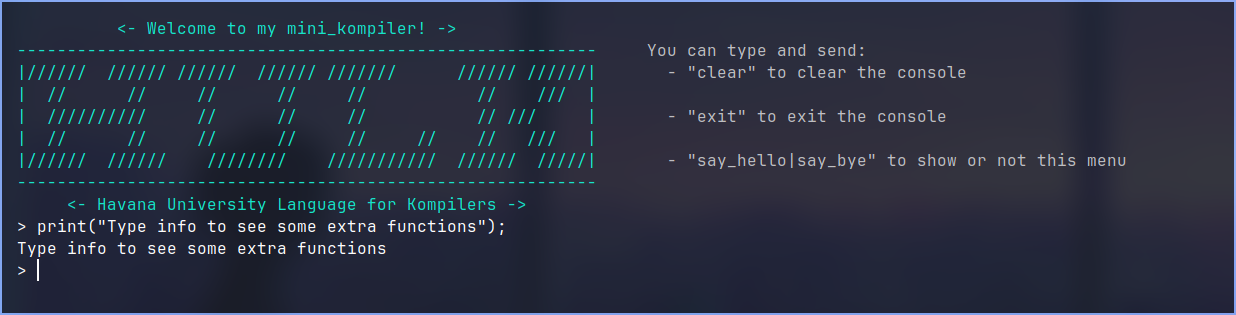
\includegraphics[width=1\textwidth]{assets/hulk_scr.png}
    \caption{Havana University Language for Kompilers}
\end{figure}
    
\subsection{Summary}
HULK (Havana University Language for Compilers) is an educational, type-safe, object-oriented and incremental programming language, designed for the Introduction to Compilers course of the Computer Science degree at the University of Havana.

A simple `Hola Mundo' in HULK looks like this:

    \hbox{print{(`Hola mundo')}}

    From a bird's eye view, HULK is an object-oriented programming language, with simple inheritance, polymorphism, and class-level encapsulation. Additionally, in HULK it is possible to define global functions outside the scope of all classes. It is also possible to define a single global expression that constitutes the entry point to the program.

    Most syntactic constructs in HULK are expressions, including conditional statements and loops. HULK is a statically typed language with optional type inference, meaning that some (or all) parts of a program can be annotated with types and the compiler will check all operations for consistency.

     But, in this case, since it is a project for 1st year students, it is a bit simplified.
     In this case, let's say, we have a one-line interpreter, which allow us, to evaluate expressions like:
     \begin{itemize}
        \item Like I said above, \hbox{print{(``Hello World'')}}
            \begin{itemize}
                \item Which is equivalent to \hbox{$print(``Hello'' + `` World'')$}
                \item And \hbox{print{(``Hello'' @ `` World'')}}
            \end{itemize}
        \item All basics `instructions' can handle simple math expressions like:
            \begin{itemize}
                \item $``2 \pm  5;''$ || $``147.6 \pm  -63;''$
                \item $``8 \times  2;''$ || $``200 \div 3;''$
                \item $``2^{64};''$ || $``sqrt(3969)'' \rightarrow  ``\sqrt{3969}''$ || $``\log(2, 10);''$
                \newpage
                \item Mathematical functions:
                    \begin{itemize}
                        \item[Sin{(x)}:] Returns the sine of x, where x is in radians. Example: Sin{(0)} returns 0.
                        \item[Cos{(x)}:] Returns the cosine of x, where x is in radians. Example: Cos{(0)} returns 1.
                        \item[Tan{(x)}:] Returns the tangent of x, where x is in radians. Example: Tan{(0)} returns 0.
                        \item[Log{(x)}:] Returns the natural logarithm (base 10) of x. Example: Log{(1)} returns 0.
                        \item[Ln{(x)}:] Returns the natural logarithm (base e) of x. Example: Ln{(1)} returns 0.
                        \item[Sqrt{(x)}:] Returns the square root of x. Example: Sqrt{(4)} returns 2.
                        \item[Abs{(x)}:] Returns the absolute value of x. Example: Abs{(-5)} returns 5.
                        \item[Pow{(x, y)}:] Returns x raised to the power of y. Example: Pow{(2, 3)} returns 8.
                        \item[Exp{(x)}:] Returns e raised to the power of x. Example: Exp{(1)} returns approximately 2.71828.
                        \item[Floor{(x)}:] Returns the largest integer less than or equal to x. Example: Floor{(1.5)} returns 1.
                        \item[Ceil{(x)}:] Returns the smallest integer greater than or equal to x. Example: Ceil{(1.5)} returns 2.
                        \item[Round{(x)}:] Rounds x to the nearest integer. Example: Round{(1.5)} returns 2.
                        \item[Rand{(min, max)}:] Returns a random integer between min (inclusive) and max (exclusive). Example: Rand{(10, 20)} returns a random number between 10 and 20.
                        \item[Factorial{(x)}:] Returns the factorial of x. Example: Factorial{(5)} returns 120.
                        \item[Fibonacci{(x)}:] Returns the xth number in the Fibonacci sequence. Example: Fibonacci{(5)} returns 5.
                        \item[IsPrime{(x)}:] Returns true if x is a prime number, false otherwise. Example: IsPrime{(5)} returns true.
                        \item[IsEven{(x)}:] Returns true if x is an even number, false otherwise. Example: IsEven{(5)} returns false.
                        \item[IsDivisible{(x, y)}:] Returns true if x is divisible by y, false otherwise. Example: IsDivisible{(10, 5)} returns true.
                        \item[IsPalindrome{(x)}:] Returns true if x is a palindrome, false otherwise. Example: IsPalindrome{(``radar'')} returns true.
                        \item[Max{(x, y)}:] Returns the maximum of x and y. Example: Max{(2, 3)} returns 3.
                        \item[Min{(x, y)}:] Returns the minimum of x and y. Example: Min{(2, 3)} returns 2.
                    \end{itemize}
                \item And thats pretty much it $\land\times \land$ 
            \end{itemize}
        \item Evaluable expressions are:
            \begin{itemize}
                \item Printing:
                    \begin{description}
                    \item[] This expression keyword receives another expressions as argument, and evaluates it, and print the returned value
                    \item[] $print(55)$; shows 55 || $print(``Kitty'')$; shows Kitty
                    \end{description}
                \item Variables:
                    \begin{description}
                        \item[] This one, contains two important keywords, ``LetKeyword'' and ``InKeyword''.
                        \item[] A basic let-in expression is: ``let $<var\_name>$ in $<statement>$''
                        \item[] Example: ``let x = ${(63 \pm 109)}^2$ in $print{(x)}$; ''
                    \end{description}
                \item Conditions:
                    \begin{description}
                        \item[] Basic and classic conditions:
                        \item[] if (condition) $<do\_if\_true>$ else $<do\_if\_false>$
                        \item[] ``if (1024 \% 2 == 0) $print(``Even'')$ else $print(``Odd'')$; ''
                    \end{description}
                \item Functions:
                    \begin{itemize}
                        \item Declare functions:
                        \begin{description}
                            \item[] To declare functions simple do:
                            \item[] function $function\_name${(arguments)} $=>$ $<statement>$;
                            \item[] Example: function Pow$(x,y)$ $=>$ $x^y$;
                            \item[] This can be used like:
                            \item[] ``let number = $Pow(2,5)$ in $print(number)$; ''
                        \end{description}
                    \end{itemize}
                \item Note: A statement is basically another instruction or expression.
            \end{itemize}
        \newpage
        \item Some expressions can be:
            \begin{enumerate}
                \item print{(``Hello World'')};
                \item print{(($({(1 + 2)} ^ 3)$ * 4) / 5)};
                \item print{($\sin{(2 * PI)}^2$ + $\cos(3 * PI / \log(4, 64))$)};
                \item function $\tan{{(x)}}$ $=>$ $\sin{{(x)}}$ / $\cos{{(x)}}$;
                \item let x = PI/2 in $print(\tan{(x)}$);
                \item let number = 42, text = ``The meaning of life is'' in print{(text @ number)};
                    \begin{itemize}
                        \item let number = 42 in (let text = ``The meaning of life is'' in (print$(text \ @ \ number)$));
                    \end{itemize}
                \item print$(7 + (let \ x = 2 \ in \ x * x))$;
                \item let a = 42 in if (a \% 2 == 0) print$(``Even'')$ else print$(``odd'')$;
                \item let a = 42 in print$(if \ (a \ \% \ 2 == 0)$ ``even'' else ``odd'');
                \item function fib$(n)$ $=>$ if (n $>$ 1) fib$(n-1)$ + fib$(n-2)$ else 1;
            \end{enumerate}
        \item And on and on, use your imagination, except if you are my programming teacher, please don't get creative, I beg you.
     \end{itemize}